\documentclass{beamer}

% This file is a solution template for:

% - Giving a talk on some subject.
% - The talk is between 15min and 45min long.
% - Style is ornate.



% Copyright 2004 by Till Tantau <tantau@users.sourceforge.net>.
%
% In principle, this file can be redistributed and/or modified under
% the terms of the GNU Public License, version 2.
%
% However, this file is supposed to be a template to be modified
% for your own needs. For this reason, if you use this file as a
% template and not specifically distribute it as part of a another
% package/program, I grant the extra permission to freely copy and
% modify this file as you see fit and even to delete this copyright
% notice. 


\mode<presentation>
{
  \usetheme{Warsaw}
  % or ...

  \setbeamercovered{transparent}
  % or whatever (possibly just delete it)
}


\usepackage[spanish]{babel}
% or whatever

\usepackage[latin1]{inputenc}
% or whatever

\usepackage{times}
\usepackage[T1]{fontenc}
% Or whatever. Note that the encoding and the font should match. If T1
% does not look nice, try deleting the line with the fontenc.


\title[Django: Framework MVC en python] % (optional, use only with long paper titles)
{Django: Framework MVC en python}

\subtitle
{El Framework para perfeccionistas con fechas limite} % (optional)

\author[] % (optional, use only with lots of authors)
{Jes�s Espino Garc�a}
% - Use the \inst{?} command only if the authors have different
%   affiliation.

\institute[GUL UC3M] % (optional, but mostly needed)
{
  GUL UC3M
}
% - Use the \inst command only if there are several affiliations.
% - Keep it simple, no one is interested in your street address.

\date[Jornadas del GUL] % (optional)
{Jornadas del GUL / 2008}

\subject{Talks}
% This is only inserted into the PDF information catalog. Can be left
% out. 



% If you have a file called "university-logo-filename.xxx", where xxx
% is a graphic format that can be processed by latex or pdflatex,
% resp., then you can add a logo as follows:

% \pgfdeclareimage[height=0.5cm]{university-logo}{university-logo-filename}
% \logo{\pgfuseimage{university-logo}}



% Delete this, if you do not want the table of contents to pop up at
% the beginning of each subsection:
\AtBeginSubsection[]
{
  \begin{frame}<beamer>{�ndice}
    \tableofcontents[currentsection,currentsubsection]
  \end{frame}
}


% If you wish to uncover everything in a step-wise fashion, uncomment
% the following command: 

%\beamerdefaultoverlayspecification{<+->}


\begin{document}

\begin{frame}
  \titlepage
\end{frame}

\begin{frame}{�ndice}
  \tableofcontents
  % You might wish to add the option [pausesections]
\end{frame}


% Since this a solution template for a generic talk, very little can
% be said about how it should be structured. However, the talk length
% of between 15min and 45min and the theme suggest that you stick to
% the following rules:  

% - Exactly two or three sections (other than the summary).
% - At *most* three subsections per section.
% - Talk about 30s to 2min per frame. So there should be between about
%   15 and 30 frames, all told.

\section{Introducci�n}

\subsection{Las cinco preguntas b�sicas}

\begin{frame}{Las cinco preguntas b�sicas}
  \begin{itemize}
    \item �Qu�?
      \begin{itemize}
      \item Framework Web.
      \item Escrito en Python.
      \item Extra�do no dise�ado.
      \end{itemize}
    \pause
    \item �Qui�n?
      \begin{itemize}
      \item Adrian Holovaty.
      \item Simon Willison.
      \end{itemize}
    \pause
    \item �D�nde?
      \begin{itemize}
      \item Lawrence, Kansas.
      \item En el peri�dico Lawrence Journal-World.
      \end{itemize}
    \pause
    \item �Cu�ndo?
      \begin{itemize}
      \item Oto�o del 2003.
      \end{itemize}
    \pause
    \item �Por qu�?
      \begin{itemize}
      \item Necesidad de cumplir unas fechas limite muy ajustadas.
      \end{itemize}
  \end{itemize}
\end{frame}

\subsection{Ventajas y Desventajas}

\begin{frame}{Ventajas}
  \begin{itemize}
    \item Es Python.
    \item Es r�pido de desarrollar.
    \item Esta pensado para la eficiencia.
    \item Es modular.
    \item Tiene muy bajo acoplamiento.
    \item Genera autom�ticamente un panel de administraci�n.
    \item Sus bibliotecas hacen gran parte del trabajo.
    \item Soporta varias bases de datos (MySQL, SQLite, Postgres, MS-SQL)
    \item Es MVC.
  \end{itemize}  
\end{frame}

\begin{frame}{Desventajas}
\begin{itemize}
  \item Es Python.
  \item No es tan simple de implantar.
  \item Es mas lento que un framework en un lenguaje compilado.
  \item No incluye AJAX de serie (todav�a).  
\end{itemize}
\end{frame}

\section{El Framework}
\subsection{MVC RoR vs MVC Django}
\begin{frame}{MVC RoR}
  \begin{itemize}
    \item Modelo: Abstracci�n del acceso a datos.
    \item Vista: Presentaci�n de los datos al usuario.
    \item Controlador: L�gica de programa.
    \item Rutas: Redirige las consultas al controlador apropiado.
  \end{itemize}  
\end{frame}

\begin{frame}{MVC Django}
  \begin{itemize}
    \item Modelo: Abstracci�n del acceso a datos.
    \item Vista: Generaci�n y presentaci�n del documento presentado al usuario.
    \item Controlador: Redirige las consultas a la vista apropiada.
    \item Plantilla: Generaci�n del HTML a partir de unos datos.
  \end{itemize}  
\end{frame}

\begin{frame}{MVC RoR vs MVC Django}
  \begin{center}
  \begin{tabular}{|ccc|}
    \hline
    RoR&&Django\\
    \hline
    Modelo&=>&Modelo\\
    Vista&=>&Plantilla\\
    Controlador&=>&Vista\\
    Rutas&=>&Controlador\\
    \hline
  \end{tabular}  
  \end{center}
\end{frame}

\subsection{Las piezas}
\begin{frame}{Esquema de consulta}
  \begin{center}
    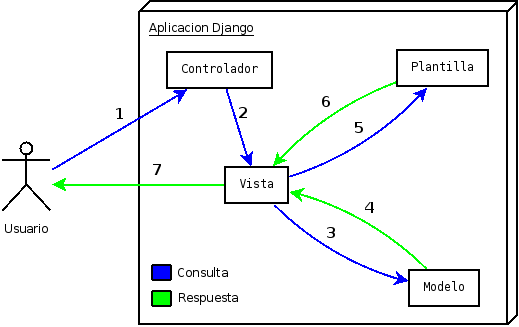
\includegraphics[width=9cm]{django-esquema.png}
  \end{center}
\end{frame}

\begin{frame}{El controlador}
  \begin{itemize}
    \item Asocia consultas (urls) a vistas.
    \item Usa expresiones regulares para determinar las equivalencias.
    \item Es capaz de capturar par�metros desde la url.
    \item El uso de expresiones regulares nos permite un primer nivel de validaci�n.
  \end{itemize}
\end{frame}

\begin{frame}{Vista}
  \begin{itemize}
    \item Ejecuta las operaciones necesarias para devolver el html al cliente.
    \item Es el encargado de la l�gica de programa.
    \item Hace uso del modelo para extraer los datos de la base de datos.
    \item Hace uso de las plantillas para generar el c�digo HTML.
  \end{itemize}
\end{frame}

\begin{frame}{Modelo}
  \begin{itemize}
    \item Define los objetos de nuestra base de datos.
    \item Permite establecer relaciones entre los objetos.
    \item Una vez definidos nos permite crearlos en nuestra base de datos.
    \item Una vez creados nuestros objetos nos permite acceder a ellos c�modamente.
  \end{itemize}
\end{frame}

\begin{frame}{Plantillas}
  \begin{itemize}
    \item Nos permiten crear la presentaci�n de los datos.
    \item Genera html a partir de un c�digo html y una serie de variables y estructuras simples.
    \item Las plantillas que incluye django soportan herencia, bucles, bifurcaciones, variables y filtros.
  \end{itemize}
\end{frame}

\begin{frame}{Middleware}
  \begin{itemize}
    \item Procesa los datos entre varios puntos del sistema.
    \item Nos permite que todas las consultas y respuestas pasen una serie de filtros.
    \item Django integra algunos como el manejo de sesiones o la autenticaci�n.
  \end{itemize}
\end{frame}

\subsection{Extras}
\begin{frame}{Interfaz de administraci�n}
  \begin{itemize}
    \item Es una aplicaci�n que viene integrada con django.
    \item Nos permite administrar nuestros objetos de la base de datos.
    \item Facilita la inserci�n de datos durante el proceso de desarrollo.
    \item Se puede personalizar, tanto el aspecto como el funcionamiento.
  \end{itemize}
\end{frame}

\begin{frame}{Vistas gen�ricas}
  \begin{itemize}
    \item Django incorpora algunas vistas gen�ricas.
    \item Nos permiten hacer las operaciones mas habituales (listar, borrar, crear...).
    \item Agilizan el proceso de desarrollo inicial.
    \item Sirven de base para crear nuestras propias vistas (a partir de ellas).
  \end{itemize}
\end{frame}

\section{Ejemplos}

\subsection{Ejemplos}

\begin{frame}{Ejemplos}
  \begin{itemize}
  \item Crear un proyecto.
  \item Crear una aplicaci�n holamundo.
  \item Hacer nuestra aplicaci�n holamundo en muchos sabores.
  \item Crear una aplicaci�n miniblog.
  \item Crear un middleware de ejemplo.
  \end{itemize}
\end{frame}

\section*{Resumen}

\begin{frame}{Resumen}
  \begin{itemize}
  \item MVC.
  \item Muy modular.
  \item Muy r�pido de programar.
  \item Muy potente.
  \end{itemize}
\end{frame}


\end{document}


